\documentclass[addpoints,12pt,answers]{exam}
\usepackage{babel}
\usepackage[top=3cm,bottom=3cm,left=2.5cm,right=2.5cm]{geometry}
\usepackage[utf8]{inputenc}
\usepackage[T1]{fontenc}
\usepackage{booktabs}
\usepackage{graphicx}
\usepackage{csquotes}
\usepackage{paralist}
\usepackage{wasysym}
\usepackage[math]{iwona}
\usepackage{setspace}
\usepackage{enumitem}
\usepackage{multirow}
%\usepackage{amsmath}



\pointpoints{Point}{Points}
\bonuspointpoints{Bonuspunkt}{Bonuspunkte}
\renewcommand{\solutiontitle}{\noindent\textbf{Solution:}\enspace}

\chqword{Frage}   
\chpgword{Seite} 
\chpword{Punkte}   
\chbpword{Bonus Points} 
\chsword{Erreicht}   
\chtword{Gesamt}

\checkboxchar{\Square}
\checkedchar{\CheckedBox}

\pagestyle{headandfoot}
%\runningheadrule
%\firstpageheader{ECO208}{Test 3}{28th Feb, 2022}
%\runningheader{ECO208}{Test 3}{28th Feb, 2022}
%\firstpagefooter{ECO208}{Test 3}{\thepage\,/\,\numpages}
%\runningfooter{ECO208}{Test 3}{\thepage\,/\,\numpages}
\doublespacing

\begin{document}
	\vspace*{3em}
	
	\makebox[\textwidth]{ECO 209  Assignment 2}
	\makebox[\textwidth]{Name:\enspace\hrulefill}
	
	\vspace*{3em}
	
	\begin{enumerate}[label=\textbf{\arabic*.}, itemsep=15pt]
		
		
		\item \textbf{(25  pts)}\label{P1}  Consider the consumption model discussed in Ch.16, the consumer has the following utility function:
		\[U = ln(c) + \beta ln(c')\]
		where $c$ is the consumption in the current period, $c'$ is the consumption in the future period and $\beta$ is the discount factor.
		
		The consumer has income of \$15,000 today and \$20,000 in the future. Also, the consumer has an initial assets ($f$) of -\$5,000 (i.e., the consumer has a debt). The consumer can save or borrow at $r= 0.02$. The discount factor ($\beta$) is equal to 0.95.
		\begin{enumerate}[label=(\alph*)]
			\item \textbf{(3  pts)} Setup the budget constraint. Shows the current period budget constraint, future period budget constraint and the lifetime budget constraint (final answer should be using the number provided).
			\item \textbf{(4  pts)} Derive the Euler equation using either substitution method or Lagrangian method. 
			\item \textbf{(4  pts)} Compute the optimal $c$ and $c'$
			\item \textbf{(3  pts)} The economy condition has changed with the interest rate $r$ rising to 0.04. What would happen to optimal level of $c$ and $c'$? Explain the intuition in 2-4 sentences.
			\item \textbf{(7  pts)} Now, the government decided to implement an income tax. It will charge $\tau y$ in the current period and $\tau y'$ in the future period. The $\tau$ is the percentage that the government is going to tax on current income $y$ and future income $y'$. Repeat part a) to part c) with this new tax policy (set $\tau$ equal to 0.05).
			\item \textbf{(4  pts)} Compare the $c$ and $c'$ in both cases (with and without tax). Explain the difference in 2-4 sentences.
		\end{enumerate}
		\clearpage
		\textbf{Solution}
		\begin{enumerate}[label=(\alph*)]
			\item Current period budget constraint: $c = 15000 +(-5000) - f'$
			
			Future period budget constraint: $c' = 20000 +f' (1+0.02)$
			
			Combine the two: $c+\frac{c'}{1+r} = 15000-5000+\frac{20000}{1.02}= 29607.84 =\bar{X}$
			
			\item Setup the Lagrangian:
			\[\ln(c) + 0.95\ln(c') + \lambda \left[ 29607.84 - c - \frac{c'}{1.02} \right]\]
			Or sub in the rearranged budget constraint $c =  29607.84 - \frac{c'}{1.02} $ into the utility function:
			
			\[\ln(29607.84 - \frac{c'}{1.02}) + 0.95\ln(c')\]
			
			The first order condition w.r.t. c':
			\[\frac{1}{c} \frac{1}{1.02} = \frac{0.95}{c'}\]
			\[\frac{c'}{c} = (0.95)(1.02) = 0.969\]
			\item 
			Rearrange the Euler equation: $	c' = 0.969 c$
			\[c^{*} + \frac{0.969c^*}{1.02}  = 29607.84\]			
			\[c^{*}   = \frac{29607.84}{1.95} = 15183.51\]			
			
			\[c^{*'} = 0.969 \times 15183.51 = 14712.82\]
			
			\item The budget constraint becomes: 
			\[c+\frac{c'}{1.04} = 15000-5000+\frac{20000}{1.04} = 29230.77\]
			The Euler equation becomes: 
			\[\frac{c'}{c} = (0.95)(1.04) = 0.988\]
			Repeat the same process above:
			\[c+\frac{0.988c}{1.04} = 29230.77 \]
			\[c^* = \frac{29230.77}{1.95} = 14990.14\]
			\[c^{'*} = 0.988 \times 14990.14 = 14810.26\]
			
			Overall, we see that the current consumption falls while the the future consumption would increase. That is because the wealth in present value has decrease as the interest rate rise (i.e., the future income worth less in term of present value). But this has the opposite effect in the future period, which lead to an increase in future consumption. 
			
			
			*If we solve the parts above using variables or parameters instead of substituting numbers, it would save a lot of time by avoiding repetitive calculations.
			
			\item The budget constraint become
			\[c=y(1-\tau) -f - f'\]
			\[c'=y'(1-\tau) +(1+r) f'\]
			\[c+\frac{c'}{1+r} = (1-\tau)y + f + \frac{(1-\tau)}{1+r} y' = \bar{X}\]
			
			Rearrange and sub it into the utility function:
			
			\[\ln(\bar{X} - \frac{c'}{1+r}) + \beta \ln(c') \]
			
			The Euler equation is:
			\[\frac{c'}{c} = (\beta) (1+r)\]
			
			Note that the Euler equation is the same, which is a property of the utility function specific in this question.
			
			Plug it into the budget constraint:
			\[c+\frac{(\beta) (1+r)}{1+r} = \bar{X}\]
			\[c_{tax} = \frac{\bar{X}}{1+\beta} = \frac{27877.45}{1.95} = 14296.13\]
			
			\[c'_{tax} = (1+r) \frac{\beta}{1+\beta} \bar{X} = 13852.95\]
			
			\item Comparing $c_{tax}$ and $c'_{tax}$ to $c$ and $c'$, the implementation of income tax by the government results in lower consumption. This is due to the fact that consumers experience a reduction in income when the government imposes an income tax, leading to a negative income effect.
		\end{enumerate}

		\clearpage
		\item \textbf{(20  pts)}\label{P2} 	Consider the consumption model discussed in Ch.16, the consumer has the following utility function:
		\[U = ln(c) + \beta ln(c')\]
		where $c$ is the consumption in the current period, $c'$ is the consumption in the future period and $\beta$ is the discount factor. The consumer can accumulate an asset amount \( f' \) in the current period to spend in the future period.
		
		The consumer has income of \$20,000 today and \$15,000 in the future. Also, the consumer has an initial assets ($f$) of \$10,000. The consumer can save or borrow at $r= 0.05$. The discount factor ($\beta$) is equal to 0.95.
		
		In this economy, the government has opted to implement a consumption tax. This tax will deduct $\tau c$ from current period income and $\tau' c'$ from future period income. Here, $\tau$ and $\tau'$ represent the rates of the consumption tax in current period and in future period.
		
		\begin{enumerate}[label=(\alph*)]
			\item \textbf{(3  pts)}  Setup the budget constraint. Shows the current period budget constraint, future period budget constraint and the lifetime budget constraint (final answer should be using the number provided).
			
			\item \textbf{(4  pts)} Derive the Euler equation using either substitution method or Lagrangian method. 
			
			\item \textbf{(3  pts)} Compute the optimal $c$ and $c'$ as a function of $\tau$ and $\tau'$
			
			\item \textbf{(3  pts)} Assuming \(\tau = \tau' = 0.05\), how would the consumer adjust their asset position in both periods (i.e., \(f\) and \(f'\))?
			
			\item \textbf{(3  pts)} The government decide to increase only $\tau$ in current period (but not $\tau'$ in future). How does it affect the optimal consumption level? 
			
			\item \textbf{(4  pts)} After a period of optimistic economic growth, it has come to an end and consumers realize that their assets are worth only \$5,000 instead of \$10,000. How might this affect their consumption behavior? Explain the intuition in 2-4 sentences.
			
			\vspace{1cm}
			
			
			
		\end{enumerate}
		
		\vfill
		
		\newpage
		
		\textbf{Solution}
		\begin{enumerate}
			\item Current period budget constraint: $(1+\tau)c = y+f-f' \to (1+\tau)c = 20,000+10,000-f'$
			
			Future period budget constraint: $(1+\tau')c'= y'+(1+r)f' \to (1+\tau')c'= 15,000+(1.05)f'$
			
			Combine the two, we have the lifetime budget constraint:
			\[(1+\tau)c +\frac{(1+\tau')c'}{1+r} = y + \frac{y'}{1+r} +f\]
			\[\to (1+\tau)c +\frac{(1+\tau')c'}{1.05} = 20000 + \frac{15000}{1.05} +10000 = 44285.71\]
			\item
			Note that $c=c(c') = \frac{1}{1+\tau}\left(44285.71 - \frac{(1+\tau')c'}{1.05} \right)$
			
			Then, $\frac{\partial c(c')}{\partial c'} = - \frac{(1+\tau')}{(1+\tau) (1.05)} $
			
			Taking derivative of the utility function, we have
			\[\frac{1}{c} \frac{\partial c(c')}{\partial c'} + 0.95 \frac{1}{c'} = 0  \]
			
			Sub in the $\frac{\partial c(c')}{\partial c'}$ and rearrange the equation, we have 
			 \[\frac{c'}{c} = \frac{1+\tau}{1+\tau'} (1.05)(0.95)\]
			 
			 *Lagrangian method would probably cleaner and easier for students who have already learn the method.
			\item Rearrange the Euler equation:
			\[c' = \frac{1+\tau}{1+\tau'} 0.9975c\]
			\clearpage
			Plug it into the budget constraint
			
			\[(1+\tau)c +\frac{(1+\tau')\frac{1+\tau}{1+\tau'} 0.9975c}{1.05} = 44285.71\]
			\[\to (1+\tau)c (1+\frac{0.9975}{1.05}) = 44285.71\]
			\[\to c = \frac{44285.71}{1.95(1+\tau)} = \frac{22710.62}{1+\tau}\]
			
			
			Sub it back to the arranged Euler equation:
			\[c' = \frac{1+\tau}{1+\tau'} 0.9975 \frac{22710.62}{1+\tau}  = \frac{22653.84}{1+\tau'}\]
			
			\item The consumer cannot change their position on the $f$ since it is determined exogenously. 
			
			Using the future period budget constraint and the optimal $c'$
			
			\[(1+0.05) \frac{22653.84}{1+0.05} = 15,000+(1.05)f'\]
			\[f' = 7,289\]
			
			This implies the consumer would use some of their asset to consume in the current period.
			
			
			
			\item According to previous answer, if $\tau$ increases while $\tau'$ remains constant, the value of $c$ would decrease, while the value of $c'$ would remain unchanged. 
			
			\item All decrease. As the $f$ decrease to 5000, there would be a negative income effect. This would lead to a decrease in both current and future consumption.
		\end{enumerate}

		\clearpage
		\item  \textbf{(12 pts)}\label{P3} 
		In the Bathtub model, the labor force $\bar{L}$ can exist in two states: employed ($E_t$) or unemployed ($U_t$) during period $t$. The evolution of unemployment over time is described by the equation:
		\[\Delta U_{t+1} = \bar{s} E_t -\bar{f} U_t\]
		where $\Delta U_{t+1}$ is the change in employment, $\bar{s}$ is the job separation rate and $\bar{f}$ is the job-finding rate.
		
		The economist has presented labor market data in the table below.
		\begin{table}[htbp]
			\centering
			\begin{tabular}{rccc}
				\toprule
				& \textbf{Separation } & \textbf{Finding } & \textbf{labour Force} \\
				&   \textbf{Rate (\%) }   &   \textbf{Rate (\%)}    & \textbf{(millions)} \\
				\midrule
				2010  & 0.24   & 4.0   & 153.9 \\
				2013  & 0.26   & 3.7   & 155.4 \\
				2015  & 0.22   & 4.4   & 157.1 \\
				2018  & 0.18   & 3.6   & 162.1 \\
				\bottomrule
			\end{tabular}%
		\end{table}%
		
		\begin{enumerate}[label=(\alph*)]
			\item \textbf{(3 pts)} Derive the steady state unemployment rate.
			\item \textbf{(2 pts)} What is the natural rate of unemployment in each of these years? 
			\item \textbf{(3 pts)} What is the number of \textit{employment} in each of these years?
			\item \textbf{(3 pts)} What would happen to the natural rate of unemployment if government implement a policy such that it would lower the separation rate. Explain using the natural rate of unemployment formula. State all the assumptions required to make a conclusion.
		\end{enumerate}
		
		\clearpage
		\textbf{Solution}
		\begin{enumerate}[label=(\alph*)]
			\item 
			
				In steady state, $\Delta U_{t+1} = 0 = \bar{s} E - \bar{f} U$. Rearrange and plug in $E = \bar{L}-U$
				\[\bar{s} (\bar{L}-U) = \bar{f} U\]
				
				Solve for $U$:
				\[U = \frac{\bar{s}\bar{L}}{\bar{s}+\bar{f}} \to u = \frac{U}{\bar{L}} = \frac{\bar{s}}{\bar{s}+\bar{f}} \]
				
			\item Apply the steady state equation derived above, 
		\begin{table}[htbp]
			\centering
			\begin{tabular}{lcccc}
				\toprule
				\textbf{Year} & \textbf{Separation} & \textbf{Finding } & \textbf{Labour Force} & \textbf{Nature Rate of } \\
				\midrule
				& \textbf{ Rate (\%)} & \textbf{Rate (\%)} & \textbf{ (millions)} & \textbf{Unemployment (\%)} \\
				\midrule
				2010  & 0.24  & 4.00  & 153.9 & 5.66 \\
				2013  & 0.26  & 3.70  & 155.4 & 6.57 \\
				2015  & 0.22  & 4.40  & 157.1 & 4.76 \\
				2018  & 0.18  & 3.60  & 162.1 & 4.76 \\
				\bottomrule
			\end{tabular}%
			\label{tab:addlabel}%
		\end{table}%
		
			
			\item 
			The employment rate is $1-u$. Multiply the labour force by it, $(1-u)L$, we can get the number of employment.
			
			\begin{table}[htbp]
				\centering
				\begin{tabular}{lccccc}
					\toprule
					\textbf{Year} & \textbf{Separation} & \textbf{Finding } & \textbf{Labour Force} & \textbf{Nature Rate of } & \textbf{Number of } \\
					\midrule
					& \textbf{ Rate (\%)} & \textbf{Rate (\%)} & \textbf{ (millions)} & \textbf{Unemployment (\%)} & \textbf{Employment} \\
					\midrule
					2010  & 0.24  & 4.00  & 153.9 & 5.66  & 145.19 \\
					2013  & 0.26  & 3.70  & 155.4 & 6.57  & 145.20 \\
					2015  & 0.22  & 4.40  & 157.1 & 4.76  & 149.62 \\
					2018  & 0.18  & 3.60  & 162.1 & 4.76  & 154.38 \\
					\bottomrule
				\end{tabular}%
			\end{table}%
			
			
			\item 	From the steady state equation, a decline in $s$ would lead to a decline in the nature rate of unemployment. 
			
%			\item 
%			\begin{itemize}
%					\item Utilization of applicant data on Online job posting platform
%					\item Utilization of past newspapers' job advertisements (e.g., situation wanted)
%				\end{itemize}
%			
			
		\end{enumerate}
		
		\clearpage 
%	\item  \textbf{(10 pts)}\label{P5} The quantity equation states that
%	\[M_t V_t = P_t Y_t\]
%	
%	
%	\begin{enumerate}[label=(\alph*)]
%		\item \textbf{(3 pts)} 	What assumptions about $M_t$, $V_t$, and $Y_t$ are necessary for the quantity theory of money to consider the money supply as the key determinant of the price level in the long run?
%		\vspace{1cm}
%		
%		%	$M_t$ is controled by the central and is exgenously given 
%		%	
%		%	$V_t$ is constant in the long run
%		%	
%		%	$Y_t$ does not affected by the money market and is determined by only the real variables, according to the classical dichotomy 
%		%	
%		%	Thus, $P_t$ is determined by the $M_t$ only
%		%	\vspace{2cm}
%		
%		\item \textbf{(2 pts)} Show that the inflation rate is a function of \textit{only} the growth rates of money supply ($g_M$) and output ($g_Y$). Make assumption if necessary. 
%		\vspace{1cm}
%		%	\[g_m + g_V = g_P + g_Y\]
%		%	Let $g_V = 0$ as it is usually assume to be a constant. Therefore,
%		%	\[g_P = \pi = g_m - g_Y\]
%		%	
%		\item \textbf{(3 pts)} Suppose the central bank announces a one-time increase in money supply to finance government's spending, followed by a sustained low growth rate of money. What are the likely effects on the inflation rate initially and in the long run?
%		\vspace{1cm}
%		
%		%	In the initial stages, the policy would lead to a very high growth rate in (\(g_m\)). According to the formula in part b), the inflation would be very high as well. However, in the long run, \(g_m\) would decrease, resulting in a lower inflation rate (\(\pi\)).
%		
%		\item \textbf{(2 pts)} If the policy was unexpected, which group of people in the economy would be hurt by this one time increase in money supply? 
%		\vspace{1cm}
%		
%		%	\begin{itemize}
%			%		\item People on fixed income
%			%		\item People hold a lot of cash
%			%		\item Lender with fixed rate
%			%	\end{itemize}
%	\end{enumerate}
		
		\clearpage 
		\item  \textbf{(30 pts)}\label{P6}  This question relates to the combined Romer and Solow  growth model discussed in Chapter 6. Holland Landing, a closed economy without government spending, features a production function:
		
		\[Y_t = A_t^{0.5} K_t^{1/4} L_{y,t}^{3/4}\]
		
		Here, \(Y_t\) represents the output, \(K_t\) denotes the capital, \(L_{y,t}\) stands for the labor employed and $A_t$ stand for TFP (or stock of ideas) in period \(t\). Holland Landing's capital accumulation follows the standard function:
		
		\[K_{t+1} = (1 - \delta) K_t + I_t\]
		
		In this equation, \(\delta\) represents the depreciation rate, and \(I_t\) represents the investment in period \(t\). The accumulation of ideas  following:
		
		\[\Delta A_{t+1} = \bar{z}L_{a,t}\]
		where $\bar{z}$ is the productivity of idea creation.
		
		The sum of numbers of workers ($L_{y,t}$) and researchers ($L_{a,y}$) equal to the total population: $L_{y,t} + L_{a,t} = \bar{N}$.  The labor supply is inelastic, with the economy consistently providing \(\bar{N}\) units of labor at any given wage.  The population is growing at the rate of $\bar{n}$. Meanwhile, there are $\ell$ proportion of the population work in the idea production. Holland Landing's population save a proportion \(\bar{s}\) of their output for investment each period.
		
		\begin{enumerate}[label=(\alph*)]
			\item \textbf{(2 pts)} Convert the production to intensive form.
			
			\item \textbf{(2 pts)} Calculate the growth rate of output per capita (y). 

			\item \textbf{(4 pts)} Show and discuss why the growth rate of output per capita ($g_y$) and capital per capita ($g_k$) are equal on the balancedgrowth path? 
			\vspace{1cm}
			
			
			\item \textbf{(3 pts)} Show that the growth rate of ideas $g_A$ is determined by constants on the balancedgrowth path.
			\vspace{1cm}
			
			\item \textbf{(3 pts)} Express $g_y$ as a function of $g_A$ on the balancedgrowth path. 
			\vspace{1cm}
			
			
			%	\item \textbf{(3 pts)} Express $g_Y$ as a function of $g_A$ on the balancedgrowth path. 
			%	\vspace{1cm}
			

			
			\item \textbf{(4 pts)}  Find the steady-state levels of \textit{output per worker}.
			\vspace{1cm}
			
			
			\item \textbf{(6 pts)} The Holland Landing government is considering promoting employment in the research and idea sector to stimulate economic growth. Draw the transition in total output $Y$ and  output per person $y$ from the balanced growth path before the policy change to after the policy change. Label all axis and key points of interest. Provide a explanation in 3-4 sentences.
			
			\vspace{1cm}
			\item \textbf{(6 pts)} (separate from part g)) The Holland Landing government is considering promoting immigration to stimulate population growth instead. Draw the transition in total output $Y$ and  output per person $y$ from the balanced growth path before the policy change to after the policy change. Label all axis and key points of interest. Provide a explanation in 3-4 sentences.
			
		\end{enumerate}
		
		\clearpage
		\begin{enumerate}[label=(\alph*)]
			\item \textbf{(2 pts)} 
			Divide the production function by $N$ and use $L_{a,t} = (1-\ell) \bar{N} \to $
			\[\frac{Y_t}{N_t} = y_t= A_t^{0.5} \frac{K_t^{1/4} L_{y,t}^{3/4}}{N_t^{1/4} N_{t}^{3/4}}  \]
			\[y_t= A_t^{0.5} k_t^{1/4} (1-\ell)^{3/4}\]
			
			\item \textbf{(2 pts)}
			Convert the production function into growth rate
			\[
			g_{yt} = 0.5 g_{At} + \frac{1}{4} g_{kt} 
			\]
			
			\item \textbf{(3 pts)} 
			
			Plug in ($I_t = s Y_t$)
			\[K_{t+1}- K_t = \Delta K_{t+1}=  sY_t -\delta K_t\]
			Divide both side by $K_t$,
			\[\frac{\Delta K_{t+1}}{K_t} = g_K  = s\frac{Y_t }{K_t}-\delta = s\frac{Y_t/L_t }{K_t/L_t}-\delta = s\frac{y_t }{k_t}-\delta\]
			Now, recall that $k_t = \frac{K_t}{L_t}$ and apply the growth rate approximate formula:
			\[g_k = g_K - g_L\]
			
			Next, plug in the $g_K$ above and the fact that $g_L = \bar{n}$
			\[g_k= \frac{\Delta k_{t+1}}{k_t} = s\frac{y_t }{k_t}-\delta - \bar{n}\]
			
			
			On the BGP, \(g_{k,t}\) is a constant, therefore, the right-hand side must also be constant. Given that \(\bar{s}\) $\bar{n}$ and \(\delta\) are constants, \(\frac{y_t}{k_t}\) must be constant. This condition is met only if \(y_t\) and \(k_t\) are growing at the same rate. If \(y_t\) were growing at a faster rate, the ratio \(\frac{y_t}{k_t}\) would increase each period. Therefore, it follows that \(g_K^* = g_Y^*\).
			
			\vspace{1cm}
			\item \textbf{(3 pts)} 	
			Researchers are used to produce new ideas:
			\[g_{At} = \frac{\Delta A_{t+1}}{A_t} =\frac{\bar{z}L_{a,t}}{A_t} \]
			Rearrange the the formula,
			\[A_t = \frac{1}{g_{A,t}} \bar{z} L_{a,t}\]
			On  the BGP, $g_{At} = g^*_{At}$, therefore, only the term $L_{a,t}$ is a variable. Apply the growth rate formula,
			
			\[g^*_{A,t} = g_{La} = \bar{n}\]
			
			Now, we know that $g_{At}$ is a constant.
			
			
			\item \textbf{(3 pts)}	
			Plug in $g_{At}=\bar{n}$, $g_K^* = g_Y^*$ into the $g_y$ equation above
			\[g_{y}^* = 0.5\bar{n} + \frac{1}{4} g_{y}^* \to g_{y}^* = \frac{4}{3} 0.5\bar{n} = \frac{2}{3} \bar{n}\]
			For the long-run combined model, this equation pins down	the growth rate of output and 	the growth rate of output per person
			
			%	\item \textbf{(3 pts)} Express $g_T$ as a function of $g_A$ on the balancedgrowth path. 
			%	\vspace{1cm}
			
			
			%	\item \textbf{(3 pts)} 
			%	
			\vspace{1cm}
			
			\clearpage
			\item \textbf{(4 pts)} 
			Use the growth rate equation derived earlier. 
			Now, we know that $g_y^*$ is a constant along a balanced growth path. This implies
			\[\frac{k^*_t}{y^*_t} = \frac{\bar{s}}{g_y^* + \delta + \bar{n}}\]
			
			Rearrange and plug it this : $k^*_t  = \frac{\bar{s}}{g_y^* + \delta + \bar{n}} y^*_t$ into the production function:
			
			\[y_t^*= A_t^{0.5} \left(\frac{\bar{s}}{g_y^* + \delta + \bar{n}} y^*_t\right)^{1/4} (1-\ell)^{3/4}\]
			\[\to y_t^{*}= A_t^{2/3} \left(\frac{\bar{s}}{g_y^* + \delta + \bar{n}} \right)^{1/3}  (1-\ell) \]
			
			\vspace{1cm}
			\item The policy would lead to an increase in \( \ell \). Initially, reallocating more labor to the research sector (\( L_{a,t} \)) from the production sector (\( L_{y,t} \)) would reduce the amount of labor available for production. As a result, both \( Y \) and \( y \) would decrease immediately.  			
			However, the long-term balanced growth path would depend on the trade-off between the reduction caused by the term \( (1-\ell) \) and the increase driven by \( A \). Assuming the net effect is positive, both \( Y_t \) and \( y_t \) would initially fall below the new balanced growth path. Over time, they would grow at an accelerated rate, eventually converging to the new balanced growth path.
			
			\textit{Extended Answer}
			
			An increase in \( \ell \) leads to a decrease in \( L_{y,t} = (1-\ell)N_t \) and an increase in \( L_{a,t} = \ell N_t \). Using the production function 
			\[
			Y_t = A_t^{1/2} K_t^{1/4} L_{y,t}^{3/4},
			\]
			The total output falls immediately as a result of the reduction in \( L_{y,t} \). Similarly, output per capita, given by $
			y_t = A_t^{0.5} k_t^{1/4} (1-\ell)^{3/4},
			$
			also decreases.
			
			Next, we analyze the growth rate and the level of the Balanced Growth Path (BGP). Using the following equations:
			\[
			g_y^* =  \frac{2}{3} \bar{n},
			\]
			\[
			y_t^* = A_t^{2/3} \left(\frac{\bar{s}}{g_y^* + \delta + \bar{n}} \right)^{1/3} (1-\ell),
			\]
			we observe that the increase in \( \ell \) does not affect the growth rate on the BGP. As a result, the slope of the BGP remains the same as before. However, \( y_t^* \) is influenced through two channels:
			\begin{enumerate}[label=(\arabic*)]
				\item A direct effect from \( \ell \), reducing \( (1-\ell) \).
				\item An indirect effect through \( A_t \), where:
				\[
				A_t = \frac{1}{g_{A,t}} \bar{z} L_{a,t}.
				\]
			\end{enumerate}
			The increase in \( L_{a,t} \) raises \( A_t \). There are two opposing forces typically assume to have an overall increase in \( y_t^* \). Consequently, the new BGP shifts upward while the slope remains the sam.e
			
			To analyze the transition from the point when the policy is implemented to the new BGP, note that both \( Y \) and \( y \) initially decrease. Using the growth rate equation for output per capita (not the BGP growth rate):
			\[
			g_{y,t} = 0.5 g_{A,t} + \frac{1}{4} g_{k,t},
			\]
			we see that \( g_{y,t} \) depends on \( g_{A,t} \) and \( g_{k,t} \), where:
			\[
			g_{A,t} = \frac{\Delta A_{t+1}}{A_t} = \frac{\bar{z} L_{a,t}}{A_t},
			\]
			\[
			g_{k,t} = \frac{\Delta k_{t+1}}{k_t} = s\frac{y_t}{k_t} - \delta - \bar{n}.
			\]
			
			Given the same \( A_t \) in period $T$, \( g_{A,t} \) increases due to the rise in \( L_{a,t} \). But, as the $A_t$ increase, the $g_{A,t}$ would slow down. Initially, \( g_{k,t} \) decreases because \( y_t \) falls, but it begins to increase as \( A_t \) grows. As a result, the transition is relative fastt at first but slows down over time. The analysis for \( Y \) is similar, with an additional population growth term in \( g_{Y,t} \), which is unaffected by the policy.
			
			\clearpage
			\begin{figure}[htbp!]
				\centering
				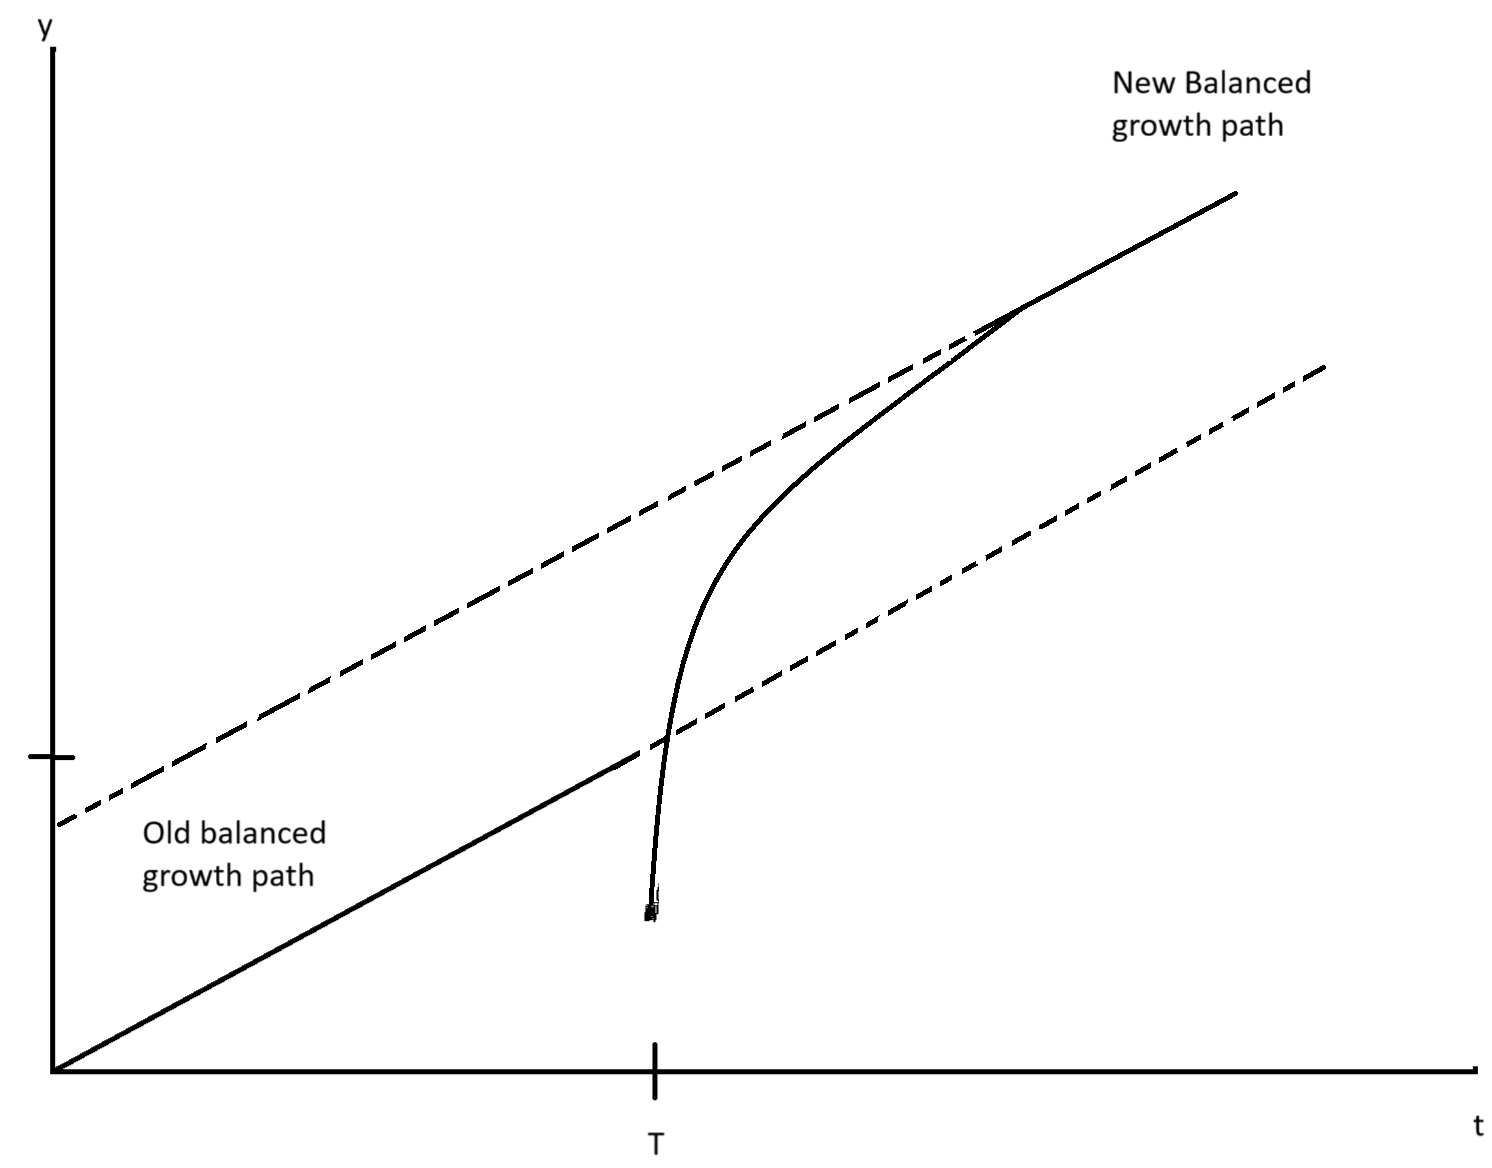
\includegraphics[width=0.7\linewidth]{figure/q6e}
			\end{figure}
			
			\begin{figure}[htbp!]
				\centering
				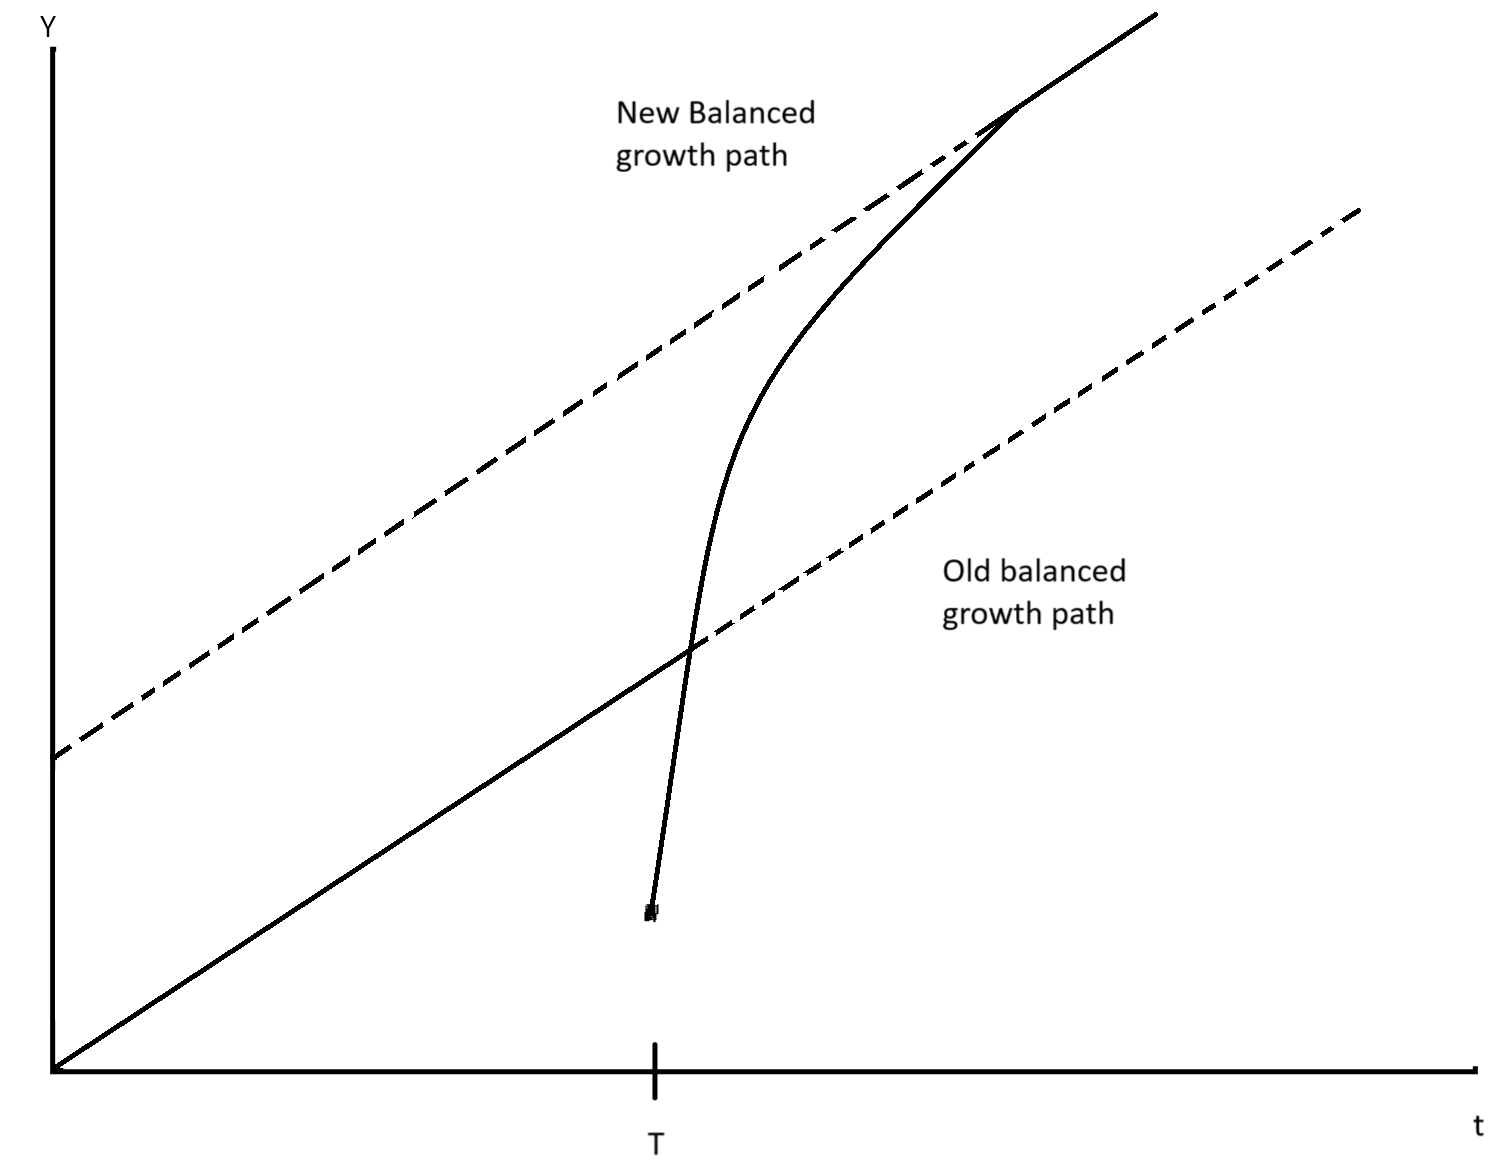
\includegraphics[width=0.7\linewidth]{figure/q6e2}
			\end{figure}
			
			\clearpage
			\item In this scenario, the government policy would result in an increase in \( \bar{n} \). This increase in \( \bar{n} \) would lead to a higher growth rate for both \( g_y \) and \( g_Y \), causing the slopes of \( Y \) and \( y \) to become steeper than before. However, the new balanced growth path (BGP) would be initially below the original BGP for a certain period because both \( g_y \) and \( \bar{n} \) have increased. Over time, the new BGP would surpass the old BGP and ultimately rise above it, as \( A_t \) grows at a faster rate.  In the graph, we assume that the growth from the increase in $\bar{n}$ outpace the slowdown from the other variables (e.g., $g_k$). The same dynamic applies to total output except that the growth should be faster than previously right away.
			
			\textit{Extended Answer}
			
			An increase in \( \bar{n} \) would have no  effect right away. Using the production function 
			\[
			Y_t = A_t^{1/2} K_t^{1/4} L_{y,t}^{3/4},
			\] 
			and
			\[y_t = A_t^{0.5} k_t^{1/4} (1-\ell)^{3/4}\]
			
			The total output and output per capita would not change at the moment $\bar{n}$ jumps up.
			
			Next, we analyze the growth rate and the level of the Balanced Growth Path (BGP). Using the following equations:
			\[
			g_y^* =  \frac{2}{3} \bar{n},
			\]
			\[
			y_t^* = A_t^{2/3} \left(\frac{\bar{s}}{g_y^* + \delta + \bar{n}} \right)^{1/3} (1-\ell),
			\]
			we observe that the increase in \( \bar{n} \) would increase the growth rate or $y$ on the BGP. As a result, the slope of the BGP become steeper. However, \( y_t^* \) is lower due to an increase in $\bar{n}$ inside the round Bracket given the same $A_t$.
				
			The increase in \( L_{a,t} \) due to an incrase in $\bar{n}$ raises \( A_t \) in the future faster than before the policy change. Consequently, the new BGP would be lower than the old BGP initially and higher than the old BGP later on, and the slope is steeper.
			
			To analyze the transition from the point when the policy is implemented to the new BGP, we  using the growth rate equation for output per capita (not the BGP growth rate):
			\[
			g_{y,t} = 0.5 g_{A,t} + \frac{1}{4} g_{k,t},
			\]
			we see that \( g_{y,t} \) depends on \( g_{A,t} \) and \( g_{k,t} \), where:
			\[
			g_{A,t} = \frac{\Delta A_{t+1}}{A_t} = \frac{\bar{z} L_{a,t}}{A_t},
			\]
			\[
			g_{k,t} = \frac{\Delta k_{t+1}}{k_t} = s\frac{y_t}{k_t} - \delta - \bar{n}.
			\]
			
			Given the same \( A_t \) in period $T$, \( g_{A,t} \) would be the same. But, as the $L_{a,t}$ rises, the $g_{A,t}$ would increase. Of course, the $A_t$ would also increase. But, from the BGP growth rate $g^*_{A,t} = g_{La} = \bar{n}$ which would be higher than before. So, $g_{A,t}$ is increasing overtime.
			
			Initially, \( g_{k,t} \) decreases because \( \bar{n} \) rise, but it begins to increase as \( A_t \) grows. Also, the $\frac{y}{k} = \frac{g_y^*+\delta+\bar{n}}{\bar{s}}$ would increase as a result of the increase in $\bar{n}$. It will eventually overcome the negative effect from the increase in $\bar{n}$ as we know $g_y^*=g_k^*$.
			
			As a result, the transition is relative slow or even negative at first but would catch up to the new BGP over time. The analysis for \( Y = yN_t \) and $g_Y = g_y + g_N$ is similar. The slope would be steeper than the case with $y$.
			
			\begin{figure}[htbp!]
				\centering
				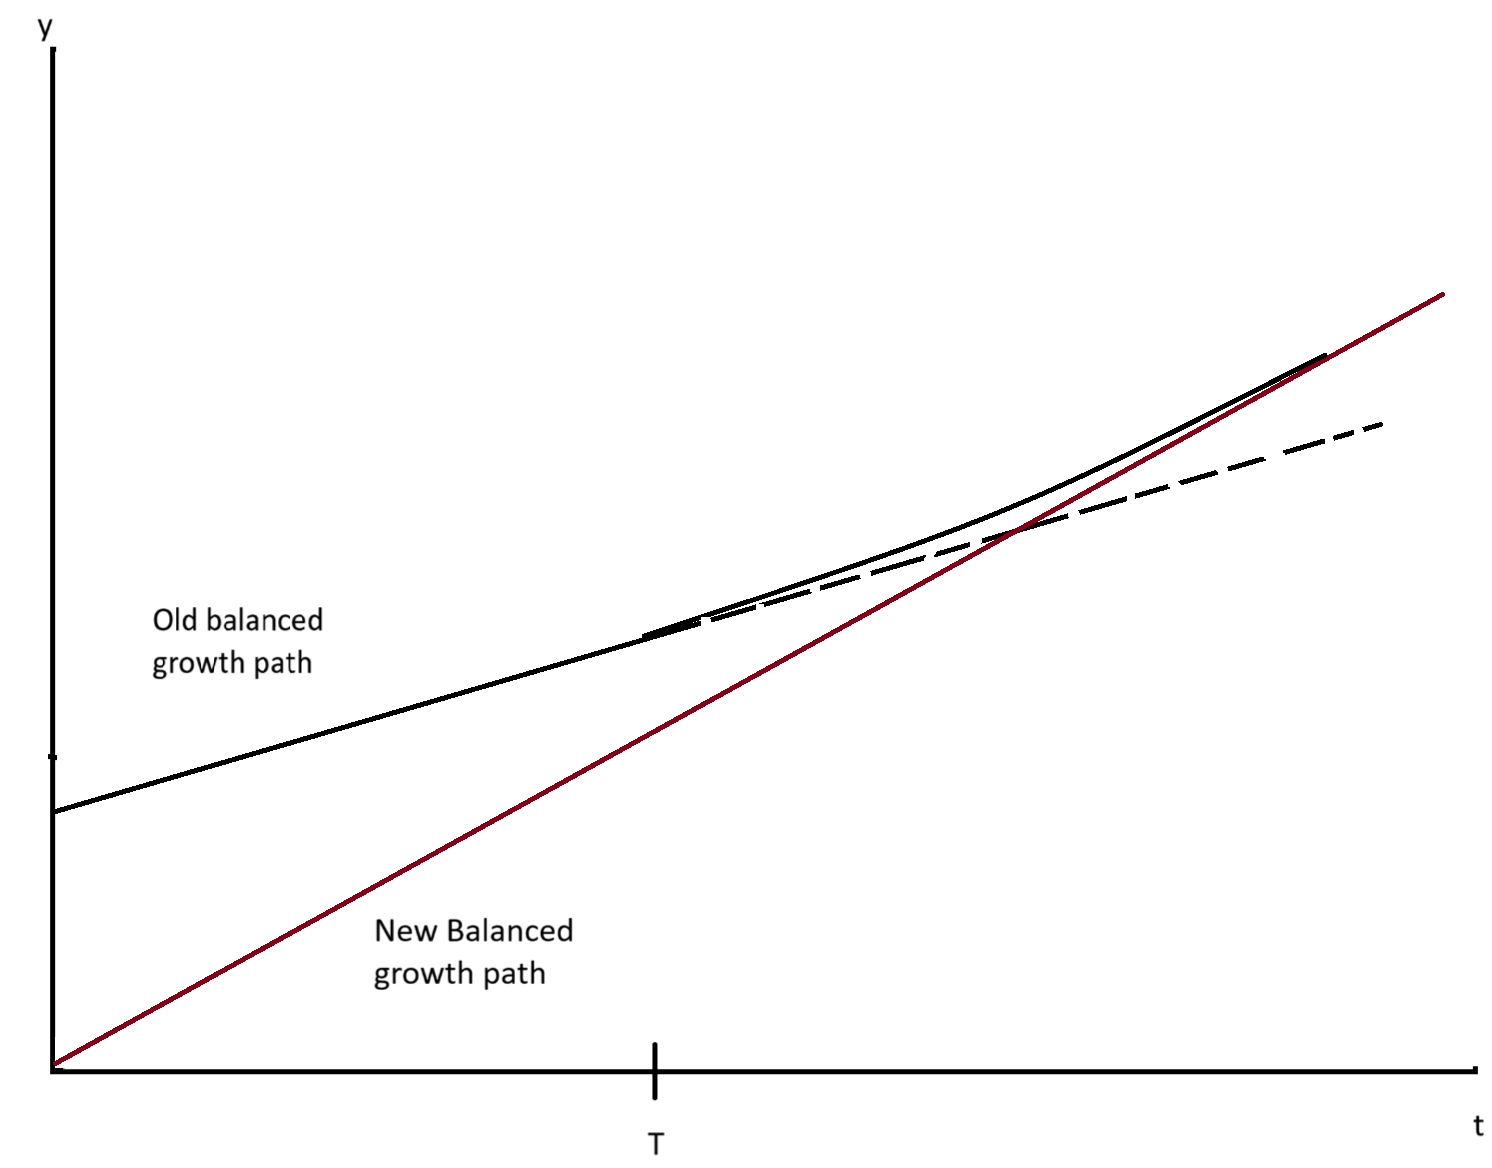
\includegraphics[width=0.45\linewidth]{figure/q6f}
			\end{figure}
			
			\begin{figure}[htbp!]
				\centering
				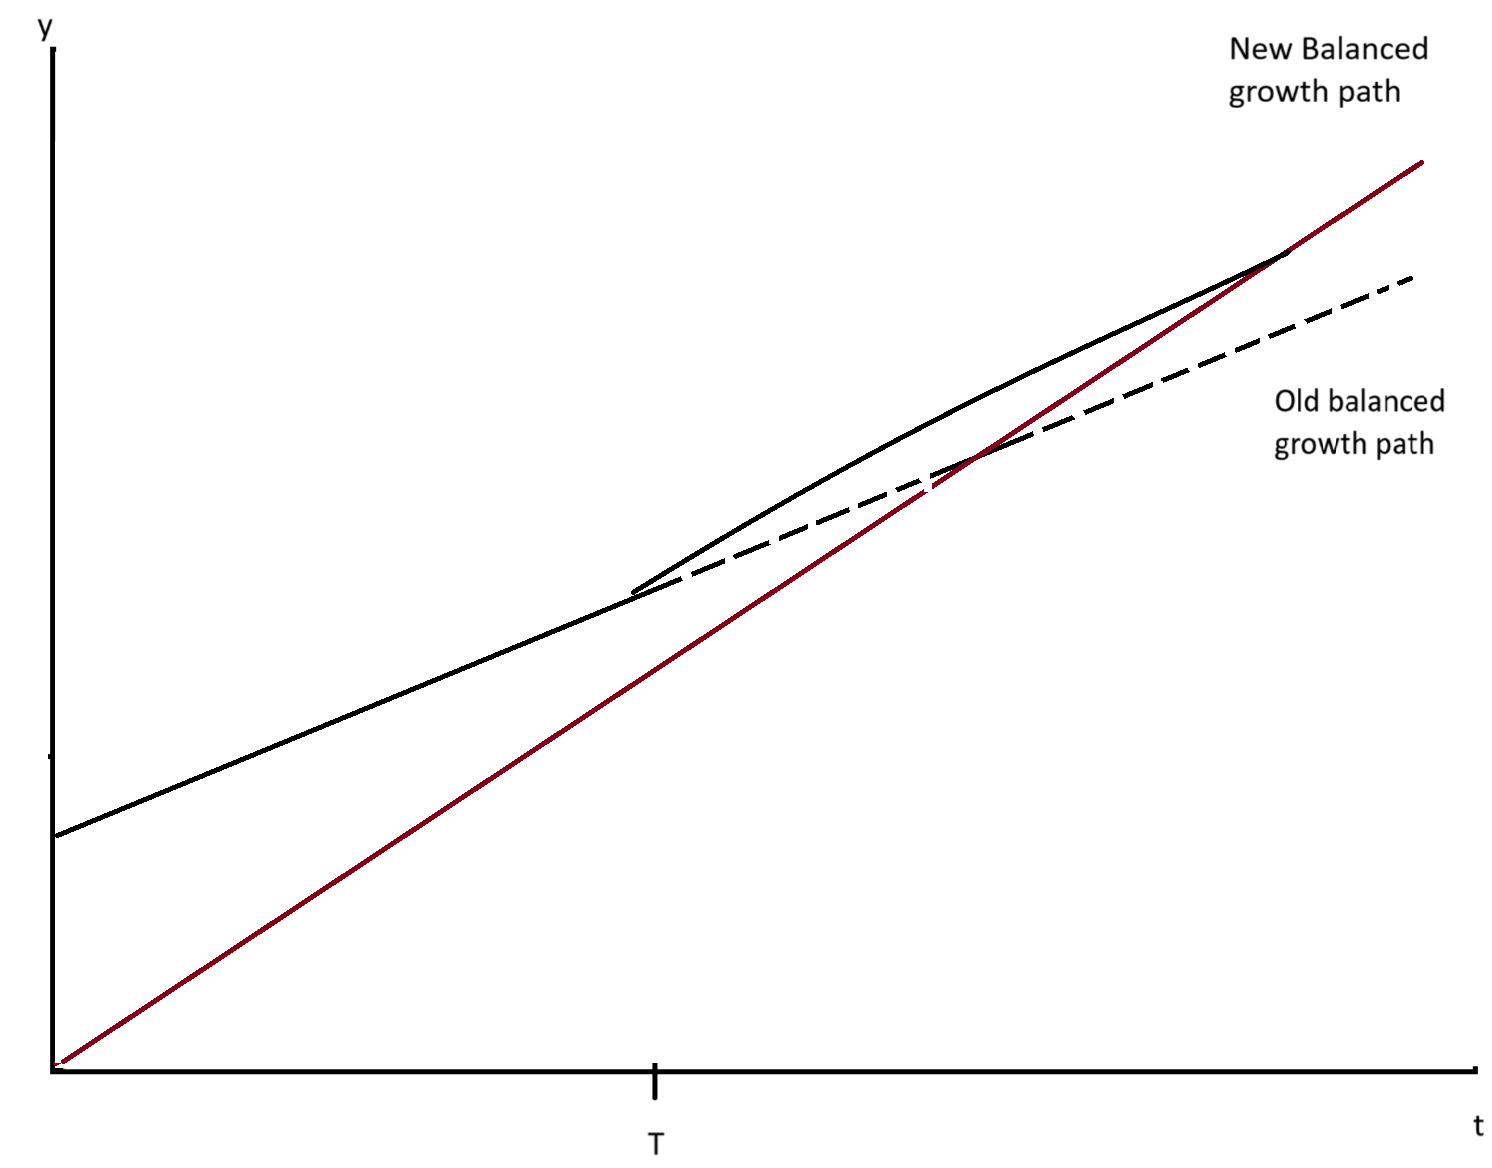
\includegraphics[width=0.45\linewidth]{figure/q6f2}
			\end{figure}
			\end{enumerate}
		
%		\newpage 
%		\centering{This page intentionally left blank.}
%		\ % The empty page
%		
		\vfill
		
		 \centering{-- The End -- }
		
		
		
		%		\begin{solution}
			%			
			%		\end{solution}	
%		\clearpage 
%		
%		\item Was wäre, wenn es keine Luft gäbe?
%		\begin{parts} 
%			\item[5] Was würde mit Luftballons geschehen? 
%			\bonuspart[6] Wie könnten Fluggesellschaften damit umgehen?
%		\end{parts}
%		
%		\item [100] Wird es morgen schneien?
%		\begin{checkboxes}
%			\CorrectChoice Ja
%			\choice Nein
%			\choice Vielleicht
%		\end{checkboxes}
%		
%		\item Ein Name der folgenden Reihe passt nicht zu den anderen. Welcher?
%		\begin{oneparchoices}
%			\choice Donald
%			\choice Dagobert
%			\choice Daisy
%			\choice Micky
%			\CorrectChoice Balu
%		\end{oneparchoices}
		
	\end{enumerate}
	
%	\begin{center}
%		\combinedgradetable[h][questions]
%	\end{center}
	
\end{document}